\documentclass{report}
\usepackage{listings}
\usepackage{graphicx}

\begin{document}
\title{Report 5 - Gaussian Blur}
\begin{figure}
    \centering
    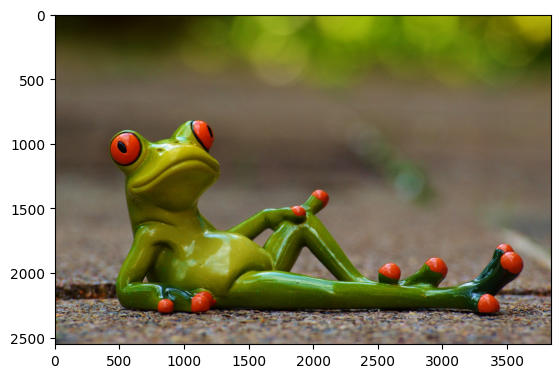
\includegraphics[width=1\linewidth]{base_frog_2D.png}
\end{figure}
\maketitle

\section{Introduction}
I'd like to say a single run on Google Colab's CPU lasted for 25min and output a black image so I didn't try a second time.

\section{Gaussian Blur on GPU}
\begin{lstlisting}[language=Python]
@cuda.jit
def GPU_Gaussian_Blur_Convolution(src, dst, matrix, matrixSum, offset):
  x = cuda.threadIdx.x + cuda.blockIdx.x * cuda.blockDim.x
  y = cuda.threadIdx.y + cuda.blockIdx.y * cuda.blockDim.y

  height = src.shape[0]
  width = src.shape[1]
  matrixSide = matrix.shape[0]

  if y < height and x < width:
    #Adressing the elephant in the room (edges), they will remain unchanged
    if y < offset or y >= (height - offset) or x < offset or x >= (width - offset):
      dst[y,x,0] = src[y,x,0]
      dst[y,x,1] = src[y,x,1]
      dst[y,x,2] = src[y,x,2]
    else:
      blur_r=blur_g=blur_b=0

      #Applying the matrix
      for ky in range(matrixSide):
        for kx in range(matrixSide):
          blur_r+=src[y+ky-offset,x+kx-offset,0]*matrix[ky,kx]
          blur_g+=src[y+ky-offset,x+kx-offset,1]*matrix[ky,kx]
          blur_b+=src[y+ky-offset,x+kx-offset,2]*matrix[ky,kx]
      dst[y,x,0]=blur_r//matrixSum
      dst[y,x,1]=blur_g//matrixSum
      dst[y,x,2]=blur_b//matrixSum

devMatrix = cuda.to_device(matrix)
devSrc = cuda.to_device(img)
devDst = cuda.device_array_like(img)

blockSide = 16
blockSize = (blockSide, blockSide)

#rounding up
gridSideX = (width+blockSide-1)//blockSide
gridSideY = (height+blockSide-1)//blockSide
gridSize = (gridSideX,gridSideY)

GPU_Gaussian_Blur_Convolution[gridSize, blockSize](devSrc, devDst, devMatrix, matrixSum, offset)
cuda.synchronize()

GPU_blurred_img = devDst.copy_to_host()
\end{lstlisting}

\begin{figure}[ht]
    \centering
    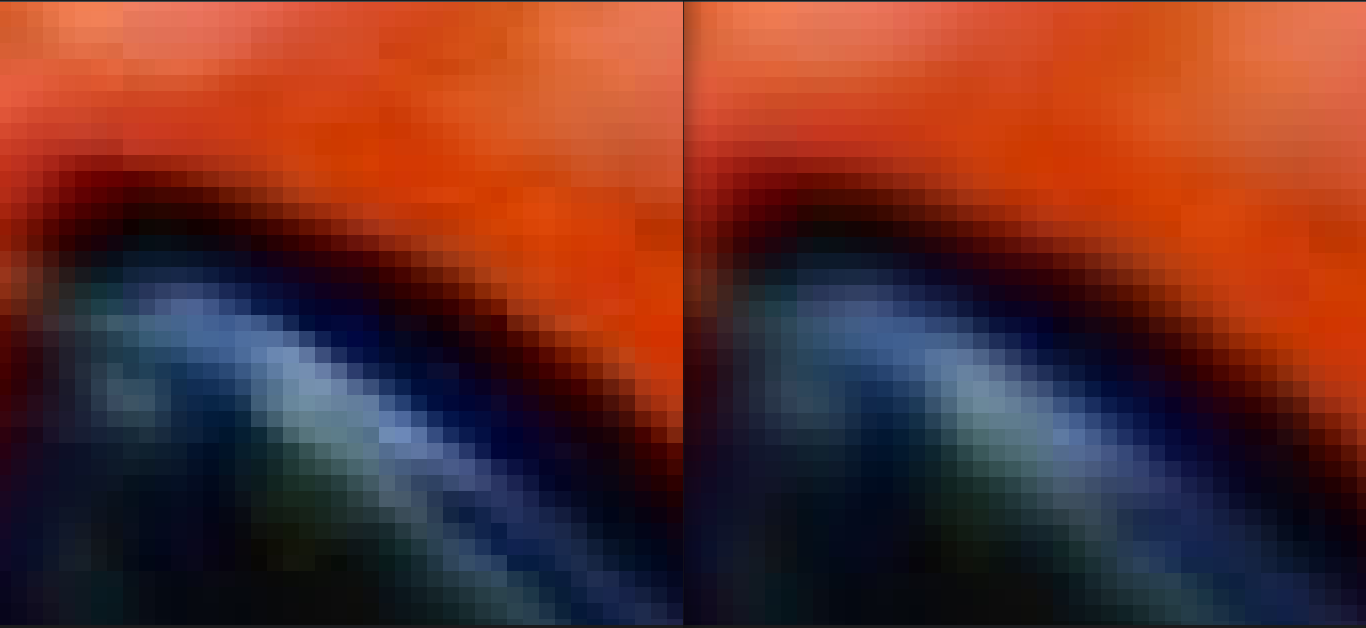
\includegraphics[width=1\linewidth]{frog_comparison.png}
\end{figure}

\section{Gaussian Blur with shared memory}
Not only we have to set variables to have global coordinates inside the GPU, but we also have to set variables to have local coordinates inside a block. 
\newline
I had to set the cuda.shared.array size fixed otherwise it was crashing. 
\newline
Same goes for numba.int32 otherwise I was having overflows.
\begin{lstlisting}[language=Python]
@cuda.jit
def GPU_Shared_Memory_Gaussian_Blur_Convolution(src, dst, matrix, matrixSum, offset):
  height = src.shape[0]
  width = src.shape[1]
  matrixSide = matrix.shape[0]

  #Where are we? Global
  tidx = cuda.threadIdx.x + cuda.blockIdx.x * cuda.blockDim.x
  tidy = cuda.threadIdx.y + cuda.blockIdx.y * cuda.blockDim.y

  #Where are we? Local
  tx = cuda.threadIdx.x
  ty = cuda.threadIdx.y

  #Initializing shared memory with fixed size
  tile_r = cuda.shared.array((16, 16), numba.int32)
  tile_g = cuda.shared.array((16, 16), numba.int32)
  tile_b = cuda.shared.array((16, 16), numba.int32)

  #Loading src data to shared memory
  if tidy < height and tidx < width:
    tile_r[ty, tx] = src[tidy, tidx, 0]
    tile_g[ty, tx] = src[tidy, tidx, 1]
    tile_b[ty, tx] = src[tidy, tidx, 2]

  cuda.syncthreads()

  if tidy < height and tidx < width:
    #Adressing the elephant in the room (edges), they will remain unchanged
    if (tidy < offset or tidy >= (height - offset) or tidx < offset or tidx >= (width - offset)):
      dst[tidy, tidx, 0] = src[tidy, tidx, 0]
      dst[tidy, tidx, 1] = src[tidy, tidx, 1]
      dst[tidy, tidx, 2] = src[tidy, tidx, 2]
      
    else:
      blur_r = blur_g = blur_b = 0

      #Applying the matrix
      for ky in range(matrixSide):
        for kx in range(matrixSide):
          s_mem_y = ty + ky - offset
          s_mem_x = tx + kx - offset

          weight = matrix[ky, kx]

          #If neighbor is in shared memory
          if 0 <= s_mem_x < 16 and 0 <= s_mem_y < 16:
            blur_r += tile_r[s_mem_y, s_mem_x] * weight
            blur_g += tile_g[s_mem_y, s_mem_x] * weight
            blur_b += tile_b[s_mem_y, s_mem_x] * weight

          #Fallback: go take it from global memory
          else:
            blur_r += (int(src[tidy + ky - offset, tidx + kx - offset, 0]) * weight)
            blur_g += (int(src[tidy + ky - offset, tidx + kx - offset, 1]) * weight)
            blur_b += (int(src[tidy + ky - offset, tidx + kx - offset, 2]) * weight)

      dst[tidy, tidx, 0] = blur_r // matrixSum
      dst[tidy, tidx, 1] = blur_g // matrixSum
      dst[tidy, tidx, 2] = blur_b // matrixSum


#Alloc and exec
devMatrix = cuda.to_device(matrix)
devSrc = cuda.to_device(img)
devDst = cuda.device_array_like(img)

blockSide = 16
blockSize = (blockSide, blockSide)

gridSideX = (width + blockSide - 1) // blockSide
gridSideY = (height + blockSide - 1) // blockSide
gridSize = (gridSideX, gridSideY)

GPU_Shared_Memory_Gaussian_Blur_Convolution[gridSize, blockSize](devSrc, devDst, devMatrix, matrixSum, offset)
cuda.synchronize()

start=time.time()
for i in range(5):
  GPU_Shared_Memory_Gaussian_Blur_Convolution[gridSize, blockSize](devSrc, devDst, devMatrix, matrixSum, offset)
cuda.synchronize()
end=time.time()
print((end-start)/5)
\end{lstlisting}

\section{Conclusion}
\begin{itemize}
    \item 0.013 - no shared memory
    \item vs.
    \item 0.018 - shared memory
\end{itemize}
\newline
Now these are weird results, I should different picture sizes and blockSizes.
I attempted with 108MP picture.
\begin{itemize}
    \item 0.10 - no shared memory
    \item vs.
    \item 0.11 - shared memory
\end{itemize}
\newline
Since the cuda shared array size has to be hardcoded, for a proper blocksize benchmark we'd need a kernel factory which sounds like overkill.
I will do it by hand.
\begin{figure}[th]
    \centering
    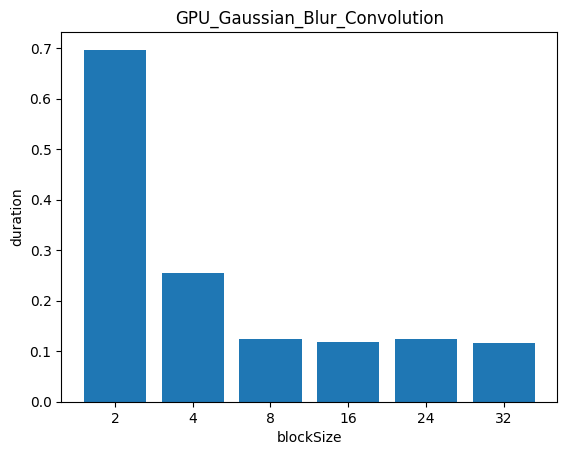
\includegraphics[width=0.75\linewidth]{barplot_blocksize_speedup.png}
\end{figure}
\end{document}